\chapter{Sumean tiivistämisen ohjelmistot\label{fuzzy-software}}

% 5

\section{Ssdeep}

Ssdeep on laajasti käytetty ohjelmisto kontekstiriippuvaisten paloittain
määriteltyjen tiivisteiden prosessointiin \citep{gayoso15}. Syötteiden
vertailu paloittain määritellyin tiivistein tapahtuu kahdessa vaiheessa.
Tiivisteet on ensin generoitava, minkä jälkeen samankaltaisuuden vertaaminen
tapahtuu tiivisteitä verraten. Ssdeepillä voidaan generoida kontekstitiippuvainen tiiviste tidostoille ja vertailla generoituja tiivisteitä keskenään.

Taulukko 3.1 havainnollistaa ssdeep-ohjelmiston käyttöä. Kahdelle
JavaScript-lähdekooditie\-dostolle generoidaan tiivisteet. Tämän
jälkeen saatuja tiivisteitä verrataan Ssdeepin vertailutilassa, joka
ilmaisee, ovatko syötteet samankaltaisia. Ssdeep määrittää samankaltaisuuden
suljetulla välillä $[0, 100]$, missä 0 tarkoittaa pienintä havaittavaa
vastaavuutta, ja 100 täydellistä vastaavuutta \citep{kornblum06}.
Mikäli Ssdeep ei kykene tulkitsemaan syötteitä samankaltaisiksi,
komento ei tulosta mitään.

\begin{table}[h]
  \caption{Alkuperäisen ja muokatun lähdekooditiedoston luonti ja vertailu ssdeep-ohjelmistolla.}
  \begin{verbatim}
   $ ssdeep -l functional.js functional-uncommented.js
  ssdeep,1.1--blocksize:hash:hash,filename
  192:eQiHcd9A+QKxYI1LIgbKvgiuqB0ML2lJGnYDTo/Z:Acd9A+QKlLpbKJ01lJQYDGZ,
    "functional.js"
  192:oQ+BA+QKNYI1LIPuiuqW0ML2lJGnYDTo/Z:KA+QKJLp01lJQYDGZ,
    "functional-uncommented.js"

  $ ssdeep -lrd functional.js functional-uncommented.js
  functional-uncommented.js matches functional.js (75)
  \end{verbatim}
\end{table}

Ssdeepin generoima tiiviste muodostuu varsinaisen tiivisteen lisäksi
lohkokoon osoittavasta kokonaisluvusta sekä syötetyn tiedoston polusta.
Lohkokoko riippuu syötteenä
annetun datan pituudesta \citep{kornblum06}. Itse tiiviste muodostuu kahdesta kaksoispisteellä erotetusta tiivisteestä.
Ssdeep iteroi syötteen uudelleen käyttäen laukaisimena kaksinkertaista
lohkokokoa. Ssdeepin tiivisteiden vertailu edellyttää, että niitä luodessa
käytetyt lohkokoot ovat yhtäsuuret \citep{kornblum06}.
 
\usetikzlibrary{shapes,arrows}
\usetikzlibrary{arrows.meta}
\tikzstyle{decision} = [diamond, draw, fill=blue!20, 
    text width=4.5em, text badly centered, node distance=3cm, inner sep=0pt]
\tikzstyle{block} = [rectangle, draw, fill=white!10,
    minimum width=12em, text centered, minimum height=2.5em]
\tikzstyle{line} = [draw, -{Stealth[length=3mm]}]
\tikzstyle{->} = [draw, -{Stealth[length=3mm]}]
    
\begin{figure}[h]
  \centering
  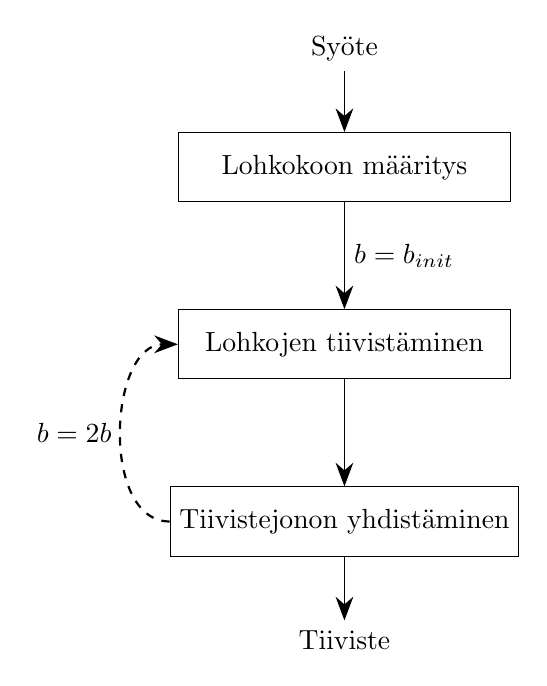
\begin{tikzpicture}[scale=3]
      \node (a) at (0, 0.25) {Syöte};
      \node [block] (b) at (0, -0.25) {Lohkokoon määritys};
      \node [block] (c) at (0, -1) {Lohkojen tiivistäminen};
      \node [block] (d) at (0, -1.75) {Tiivistejonon yhdistäminen};
      \node  (e) at (0, -2.25) {Tiiviste};
      \path [line] (a) -- (b);
      \path [line] (c) -- (d);
      \path [line] (b) -- (c) node[midway,right] {$b=b_{init}$};
      \path [line] (d) -- (e);
      \draw [->, dashed, thick] (d) to [out=180, in=180] node[midway, left] {$b=2b$} (c);
  \end{tikzpicture}
  \caption{Kontekstiriippuvaisen paloittain määritellyn tiivisteen luonti Ssdeep-ohjelmistossa.}
\end{figure}

Ssdeep käyttää kontekstin tunnistamiseen monen kontekstiriippuvaisen
tiivistealgoritmin tavoin rekursiivista tiivisitettä \citep{kornblum06}.
Syötettä iteroidessasan Ssdeep käyttää rekursiivista tiivistettä pitääkseen
yllä tilaa viimeisimmin käsiteltyjen alkioiden muodostamasta kontekstista.
Rekursiivista tiivistettä käytettäessä on yleensä määritetly myös niin sanottu
laukaisinarvo, johon rekursiivista tiivistettä verrataan. Laukaisinarvoa
vastaava rekursiivisesti määritetlty tiiviste ilmaisee vallitsevan kontekstin
vaihtumisen. Kontekstin ilmaiseva tiiviste $h$ voidaan esittää tiivistefunktion
$R$ rekursiivisena kutsuna

\[
  h = R(a_i, R(a_{i - 1}, R(a_{i - 2}, \dots, R(a_{i - n + 1}) \dots))),
\]                                                                     

missä $i$ on haluttu syötteen indeksi ja $n$ huomioitavien alkioiden määrä.
Edellinen lauseke ei ole kuitenkaan tehokas tapa laskea tiivistettä. Käytännön
sovelluksissa riittävää on tiivistää nykyinen alkio sekä edellisten alkioiden tiiviste, josta poistetaan varhaisimman alkion vaikutus algoritmista riippuen esimerkiksi
bittioperaatiolla. Ssdeepissä tiivistykseen käytetään Adler32-tiivistefunktiota \citep{kornblum06}.

\section{Sdhash}

Sdhash on epätodennäköisiä ominaisuuksia tiivistävä ohjelmisto sumeiden tiivisteiden
prosessointiin. Sdhash kuuluu tiivistettyihin ominaisuusjonoihin \parencite{martin-perez21}.
\textcite{naik19} mainitsevat Sdhashin perustuvan väitteelle, jonka mukaan kaikilla syötteille
on tieyttyjä tilastollisia ominaisuuksia. Osa syötteen ominaisuuksista on erityisen epätodennäköisesti ilmeneviä. Datan identiteetin säílymisen kannalta ominaisuuksista valitaan epätodennäköisimmin
ilmenevät. Mitä useampi epätodennäköisesti ilmenevevä ominaisuus ilmenee toisessa syötteessä,
sitä suuremmalla todennäköisyydeellä niiden alkuperä on sama. 

\begin{figure}[h]
 \centering
  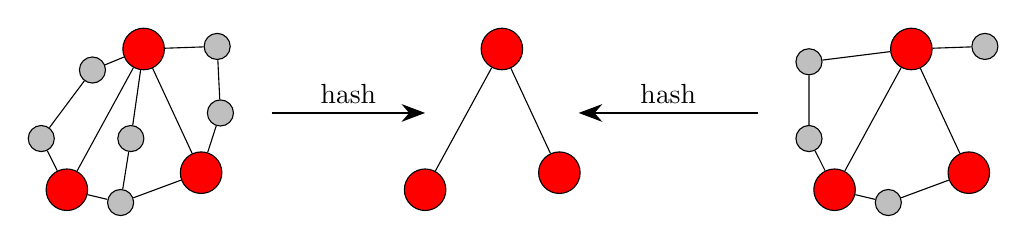
\begin{tikzpicture}[scale=0.65]
    \node[circle, draw, fill=lightgray, minimum size=0.75em] (a) at (-1.45, -0.25) {};
    \node[circle, draw, fill=lightgray, minimum size=0.1em] (b) at (-3, 1) {};
    \node[circle, draw, fill=lightgray, minimum size=0.5] (c) at (0.437, 2.8) {};
    \node[circle, draw, fill=lightgray, minimum size=0.3] (d) at (-2, 2.339) {};
    \node[circle, draw, fill=red, minimum size=1.5em] (e) at (0.123, 0.333) {};
    \node[circle, draw, fill=red, minimum size=1.5em] (f) at (-1, 2.75) {};
    \node[circle, draw, fill=red, minimum size=1.5em] (g) at (-2.5, 0) {};
    \node[circle, draw, fill=lightgray, minimum size=0.75] (h) at (-1.25, 1) {};
    \node[circle, draw, fill=lightgray, minimum size=1.25] (i) at (0.5, 1.5) {};

    \path [line] (11, 1.5) -- (7.5, 1.5) node [midway, above] {hash};
    \node[circle, draw, fill=red, minimum size=1.5em] (e2) at (7.123, 0.333) {};
    \node[circle, draw, fill=red, minimum size=1.5em] (f2) at (6, 2.75) {};
    \node[circle, draw, fill=red, minimum size=1.5em] (g2) at (4.5, 0) {};

    \path [line] (1.5, 1.5) -- (4.5, 1.5) node [midway, above] {hash};
    \node[circle, draw, fill=lightgray, minimum size=0.75em] (a3) at (13.55, -0.25) {};
    \node[circle, draw, fill=lightgray, minimum size=0.1em] (b3) at (12, 1) {};
    \node[circle, draw, fill=lightgray, minimum size=0.5] (c3) at (15.437, 2.8) {};
    \node[circle, draw, fill=lightgray, minimum size=0.3] (d3) at (12, 2.5) {};
    \node[circle, draw, fill=red, minimum size=1.5em] (e3) at (15.123, 0.333) {};
    \node[circle, draw, fill=red, minimum size=1.5em] (f3) at (14, 2.75) {};
    \node[circle, draw, fill=red, minimum size=1.5em] (g3) at (12.5, 0) {};

    \path [line] (e3) edge[-] (f3) {};
    \path [line] (f3) edge[-] (g3) {};
    \path [line] (e3) edge[-] (a3) {};
    \path [line] (g3) edge[-] (a3) {};
    \path [line] (g3) edge[-] (b3) {};
    \path [line] (f3) edge[-] (c3) {};
    \path [line] (f3) edge[-] (d3) {};
    \path [line] (d3) edge[-] (b3) {};

    \path [line] (e2) edge[-] (f2) {};
    \path [line] (f2) edge[-] (g2) {};

    \path [line] (e) edge[-] (f) {};
    \path [line] (f) edge[-] (g) {};
    \path [line] (e) edge[-] (a) {};
    \path [line] (g) edge[-] (a) {};
    \path [line] (g) edge[-] (b) {};
    \path [line] (f) edge[-] (c) {};
    \path [line] (f) edge[-] (d) {};
    \path [line] (e) edge[-] (i) {};
    \path [line] (i) edge[-] (c) {};
    \path [line] (d) edge[-] (b) {};
    \path [line] (h) edge[-] (a) {};
    \path [line] (h) edge[-] (f) {};

  \end{tikzpicture}
  \caption{Kaksi samasta verkosta erisuuriksi muokattua verkkoa tiivistetään samaksi tiivisteeksi valitsemalla ainoastaam poikkeavat eli suuremmeat alkiot.}
\end{figure}

Sdhashin ominaisuudet ovat 64 tavun merkkijonoja \citep{roussev10}. Tiivisteen generoinnin aikana Sdhash käy
läpi syötteen kaikki ominaisuudet valiten niistä epätodennäköisimmät.
Jokaiselle syötteen ominaisuudelle määritetään entropia-arvo.
Syötteen ominaisuuksille generoidaan presedenssiarvo perustuen entropia-arvoon.
Populaariarvon laskemiminen vaatii syötteen läpikäyntiä käyttäen ikkunaa, joka
rajaa sisälleen $W$ syötteen ominaisuutta. Ikkunaa liu'utetaan ominaisuus
kerrallaan eteenpäin, ja jokaisen ominaisuuden kohdalla valitaan pienimmästä
indeksistä katsottuna ikkunan pienin presedenssiarvo. Valitun arvon kohdalla
olevan ominaisuuden populaariarvoa kasvatetaan yhdellä.

Syötteen iteroimisen jälkeen ominaisuuksista valitaan ne, joiden populaariarvolle
pätee $R_{pop} >= t$, missä $t$ on algoritmille määritelty raja-arvo. Valituilla
ominaisuuksilla katsotaan olevan tilastollisesti pieni todennäköisyys esiintyä
sattumanvaraisessa syötteessä. Valitut ominaisuudet tiivistetään
SHA-1-tiivistefunktiolla tallettavaksi generoitavaan tiiviisteeseen.
Tiivistetyt ominaisuudet talletetaan Bloom-suodattimeen, joista
muodostetaan tiiviste yhdistämällä suodattimet jonoksi.
Bloom-suodattimella esitettävään joukkoon voidaan lisätä alkiota sekä tarkistaa,
kuuluuko alkio joukkoon. Suodatin totetutetaan bittijonona, jonka permutaatiot
kuvaavat joukkoon kuuluvia alkiota. Syötteille yhteisten ominaisuuksien määrä
on selvitettävissä laskemalla suodatinten välinen Hamming-etäisyys.

Sdhashissa ilmenee Bloom-suodattimesta johtuvia aiheettomia
osumia. Suorituskyyvn optimointi heikentää tarkkuutta,
ja suodatin saattaa virheellisesti tulkita tuntemattoman
alkion kuuluvan joukkoon. Jokainen bitti kuvaa useampaa kuin yhtä
permutaatiota, joten useampi bittipermutaatio saattaa
samanaikaisesti kuvata myös muita, joukkoon kuulumattomia
alkioita. Aiheettomat osumat eivät käytännössä aiheuta tuloksiin merkityksellisiä muutoksia.

\textcite{breitinger12} mainitsevat Sdhashin vahvuutena olevan katkelmien havaitseminen syötteestä
tiedostojen vertaamisen sijaan.

\section{Mvhash-b}

Mvhash-b on Ssdeepistä ja Sdhashista poikkeava ohjelmisto, jonka toimintaperiaate
perustuu tavujonojen esiintyvyyteen \parencite{martin-perez21}. Mvhash-b ei
tarkastele syötettä lohkoina.

Mvhash-b vertaa syötteen jokaisen indeksin $k$ $n$-naapuruston
tavujen 1-bittien lukumäärää $bitcount(N_{k,n})$ raja-arvoon $t$.
Mikäli $bitcount(N_{k,n}) \leq t$, asetetaan tavu $B_k = 255$.
Muutoin asetetaan $B_k = 0$. Raja-arvoksi on määritelty lukumäärä,
joka kattaa $n$-naapurustossa bittien enemmistön. Näin syntyy
eri mittaisia tavujonoja, jotka sisältävät vuorotellen
joko arvon 0 tai 255. Enemmistö kuvaa kyseisten alkioiden
yleistä tilaa, joka pysyy tiettyissä rajoissa ennallaan
muutoksista riippumatta.

Tavujen mukauttamisen jälkeen syöte muodostuu $m$ tavun jonoista,
joissa kaikkien tavujen arvo on 0 tai 255. Tällaiset tavujonot
$B = b_0, b_1,b_2, \dots, b_n$ voidaan esittää RLE-koodattuna
tavujen arvon sekä lukumäärän järjestettynä parina. RLE-koodauksen
muodostama jono talletetaan Sdhashin tavoin Bloom-suodattimeen.
Tiiviste muodostuu Bloom-suodattimesta, ja samankaltaisuus
määritetään kahden tiivisteen välisenä Hamming-etäisyytenä.
Erityisesti kaikkia suodattimia on verrattava kaikkiin,
koska syötteen pituuden muutokset saattavat siirtää
ominaisuuksia toiseen suodattimeen \parencite{breitinger13}.

Mvhash-b:n pisteytysjärjestelemä poikkeaa Ssdeepin ja Sdhashin
vastaavista. Kaikkissa samankaltaisuutta kuvataan suljetulla
välillä $[0, 100]$, mutta asteikko on Mvhash-b:ssä käänteinen
luvun 0 kuvatessa täydellistä vastaavuutta, eli Hamming-etäisyyttä 0.
